\chapter{Task Selection and Patient “Pick-up"} 

% \begin{tabular}{c}
    \textbf{Task Selection and Patient “Pick-up" -- How Familiarity Encourages Physician Multitasking in the Emergency Department.}
    This Chapter is co-authored with Dr. Diwas KC (Emory University) and Dr. Bradley Staats.
% \end{tabular}

% \begin{center} \rule{6in}{0.01in} \end{center}
% \noindent
%  \textbf{Chapter Abstract:} \\
%  \textbf{Background:} Patient demand for emergency medical services continues to rise from all-time highs. Physicians generally respond to the rising demand by increasing their level of multitasking. \\
%  \textbf{Aim:} What leads Emergency Department physicians to select which patients, and how many patients, they will treat? Queuing models frequently assume individual servers operate independently of other servers. In contrast, we consider how familiarity between peer physicians affects patient selection and the chosen multitasking level, a process more commonly known in the ED as “patient pick-up." \\
%  \textbf{Methods:} Using empirical observations from two Emergency Departments, we explore whether familiarity alters patient pick-up behavior, we determine the effect of familiarity on multitasking, and we measure the combined impact of familiarity and multitasking on other ED outcomes. \\
%  \textbf{Results:} Among ED physicians, greater average familiarity leads to an increase in patient pick-up rate, observed multitasking, and shorter patient wait time -- with no identifiable, negative impact to patient processing time or length of stay. Moreover, the effects intensify at the end of a physician’s shift and for patients in severe condition. \\ 
%  \textbf{Conclusion:} Within more familiar groups, physicians appear willing to exert more effort. Our study explicates how the benefits materialize and illustrates why researchers must consider server familiarity moving forward.
% \begin{center} \rule{6in}{0.01in} \end{center}
% \noindent\keywords{Healthcare, Discretion, Productivity, Familiarity, Empirical Operations} \\

\section{Introduction} 
\begin{quote}
    \textit{Two are better than one, because they have a good reward for their toil. \\
    For if they fall, one will lift up the other.} \\
    (Jewish Proverb) % \medskip
\end{quote}

 Patient demand for emergency medical services has never been greater. In the U.S., as fewer people access medical care through a primary care provider, more people access care through the hospital emergency department, or ED \citep{Greenwood-Ericksen2019,Ganguli2020}. Between 1993 and 2006 the proportion of hospital patients admitted through the ED rose by more than 30\% \citep{Schurr2012}. And though structural reductions in overcrowding can yield significant health benefits \citep{Woodworth2019}, usually ED physicians must simply “do more, with less." And so the physicians respond by increasing their level of multitasking, an important driver of operational performance in service operations and queuing systems \citep[][]{KC2014,KC2020_productivity}.
 
 Unlike other types of queuing systems, however, the ED allows physicians discretion in task selection \citep{KC2020_tcp}. That is, ED queues do not operate solely under a policy of “first-come, first-served, by severity;" such a setup yields significant productivity benefits over alternatives \citep{Chan2016}. What, then, leads physicians to select which patients, and how many patients, they will treat? For one, strong intrinsic motivation drives many clinicians to serve \citep{Madara2015}. But there are also pressures to perform \citep{Mas2009} and temptations to slack-off \citep{Karau1993}. The ED also epitomizes an environment of social exchange \citep{Homans1961,Blau1964} and reciprocity \citep{Gouldner1960}: “I'll take this patient if you take the next one." One aspect common in all such contexts is coworker \textit{familiarity}. In our study, we consider how familiarity between peer physicians in the ED affects patient selection and the chosen multitasking level, a process more commonly known as “patient pick-up."
 
 As highlighted by \cite{Boudreau2003}, queuing models in operations frequently assume servers operate independently of one another: “The hope is always that what is ‘assumed away’ is not critical to the research questions under study” \citep[p. 740]{Bendoly2006}. But gaps between models and real-world data \citep[e.g.,][]{Ouyang2021} may arise from assumptions \citep{Bendoly2010}, especially the “independent server" assumption \citep{Schultz1997}. If coworker familiarity affects a decision to multitask -- when we assume servers operate independently -- then such an assumption may not be tenable here. Familiarity does impact other operational outcomes such as service rate \citep[e.g.,][]{Reagans2005} and team performance \citep[e.g.,][]{Huckman2011}. And physicians have told us: “If I'm working alongside someone I know to be `Dr. Idler' ... I might alter my typical approach to patient pick-up." This paper questions the assumption of exogeneity among parallel servers and considers whether inter-server dependence (e.g., familiarity) impacts ED performance.

\begin{figure}[!b]
     \centering
     \caption{Average physician multitasking (i.e., patient load) increases with greater familiarity.} \medskip
     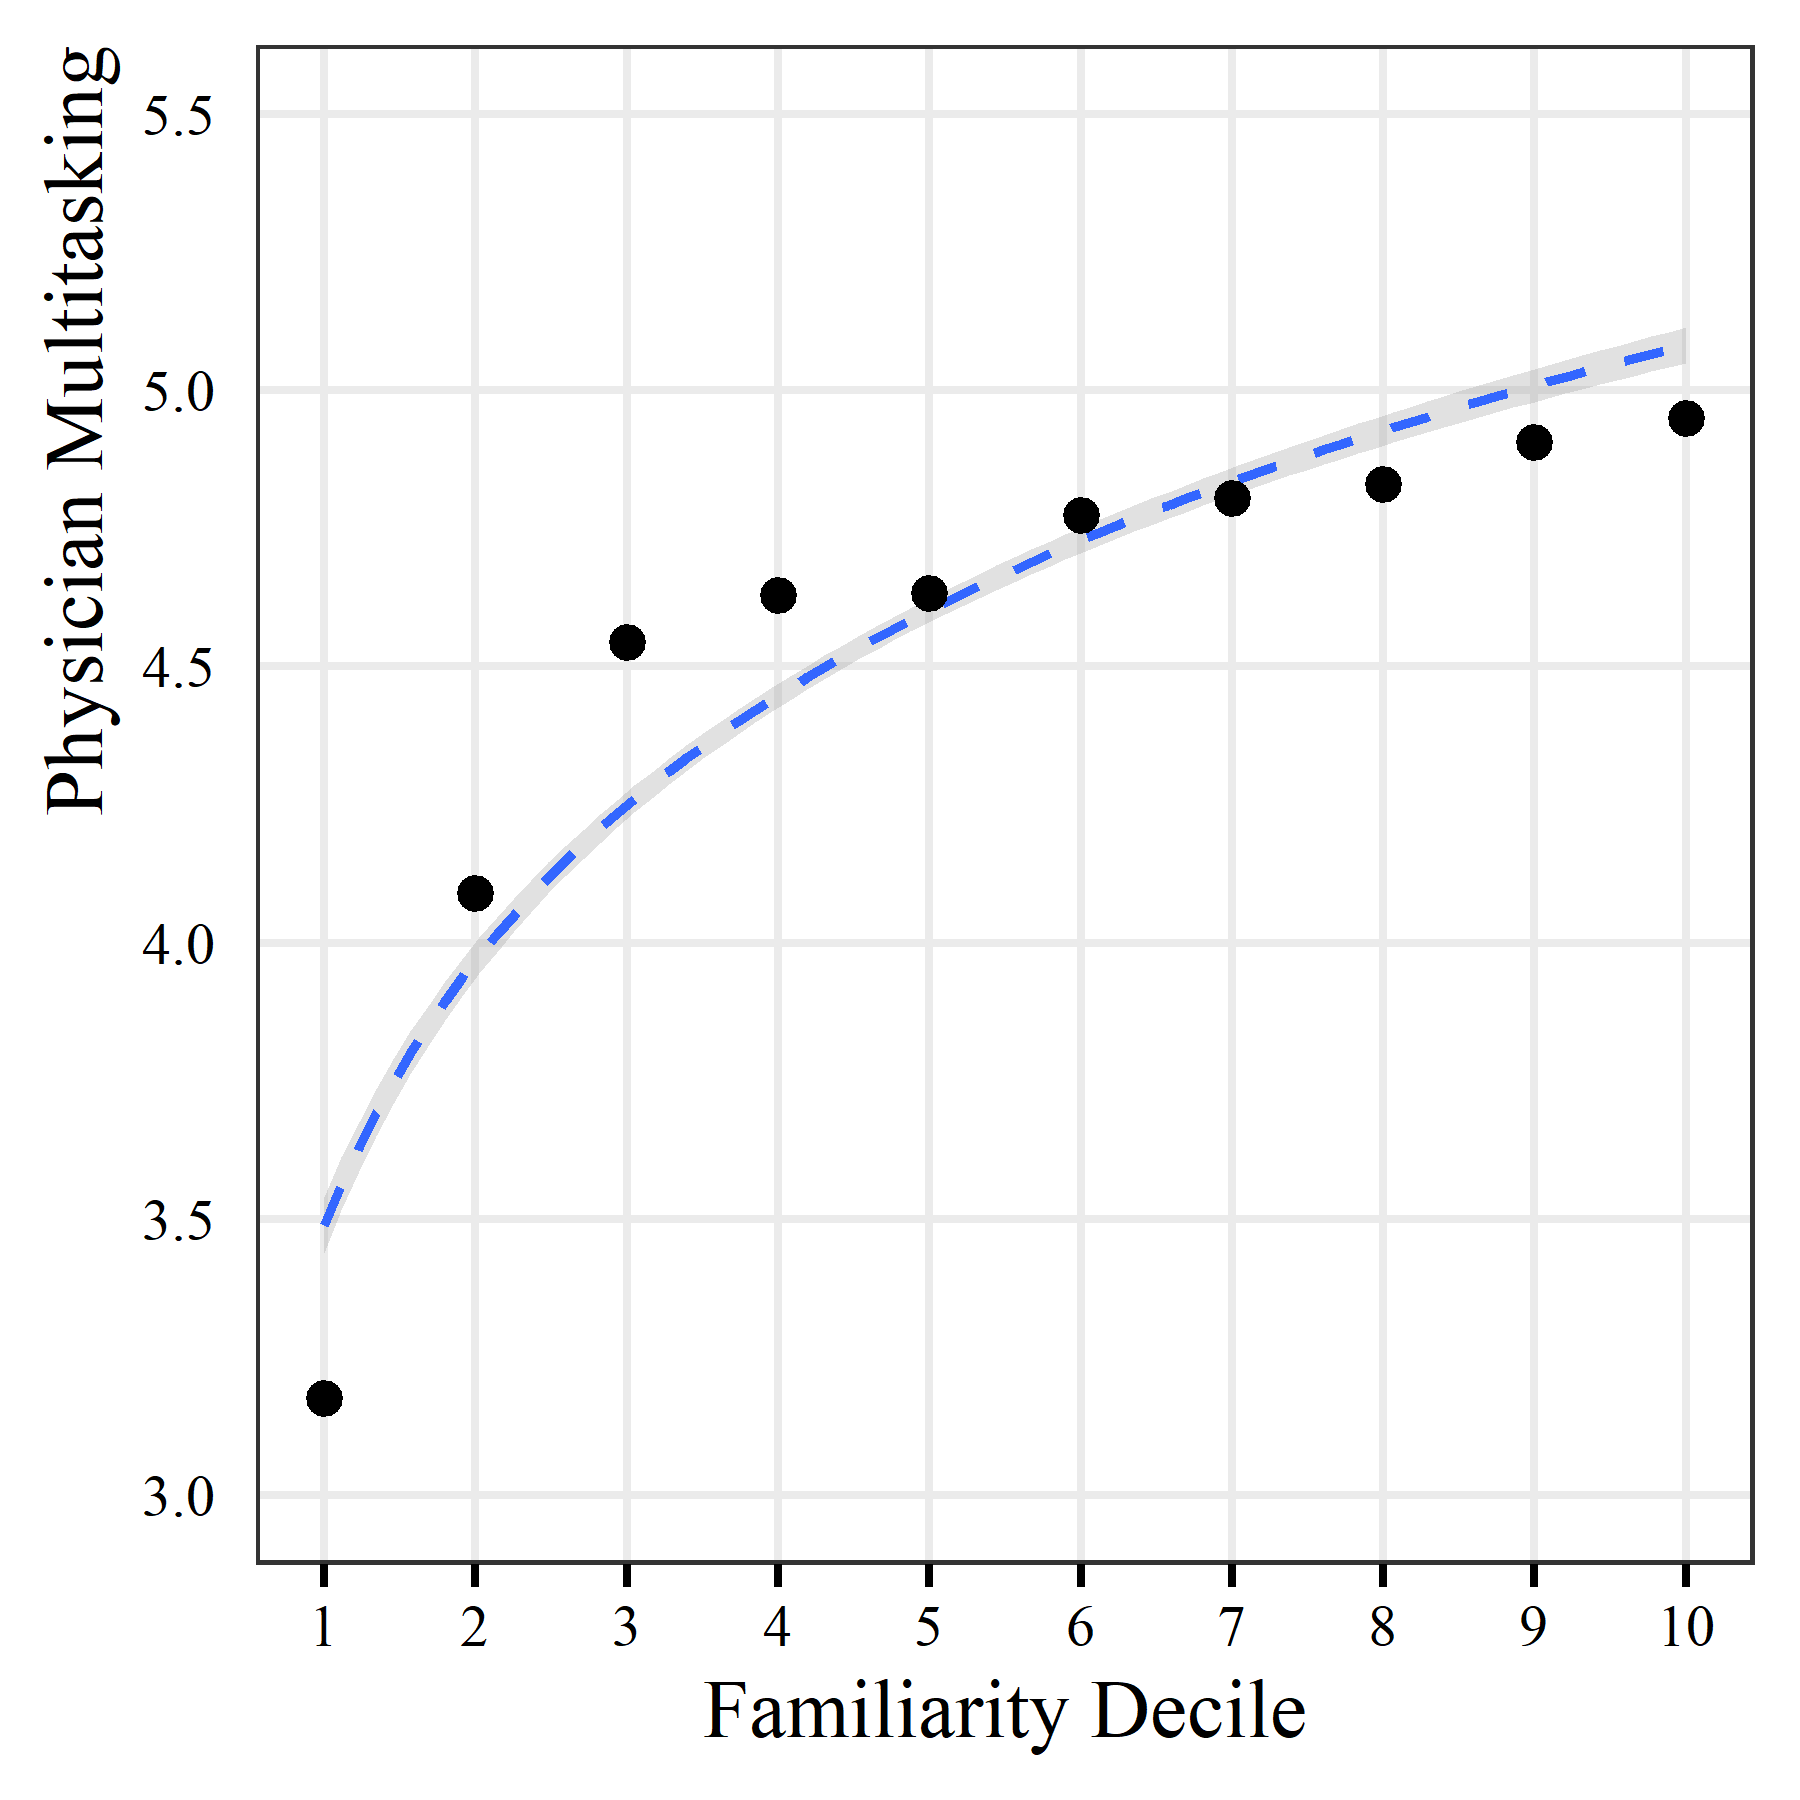
\includegraphics[scale=1]{Figures/PU/Load v. Fam (Xtile).png}     
     \label{fig:load_fam}
    %  \floatfoot{\textit{Figure Note:} Logarithmic smoothing trend plotted in blue. }
 \end{figure}

 We seek to answer the following research questions. First: When picking up patients from a common pool, does familiarity among ED physicians alter the patient pick-up process? A physician initiates “patient pick-up" when she selects a waiting patient and begin treatment (see full discussion in Section \ref{emp_context}). Second: Does familiarity among ED physicians alter multitasking behavior? And finally: What other ED factors change with familiarity and altered pick-up decisions? Using observations from two EDs, Figure \ref{fig:load_fam} motivates our research questions. Observe higher familiarity deciles correspond to greater levels of physician multitasking, measured as “the number of distinct patients cared for by a physician at a given point in time" \citep[p. 169]{KC2014}. Building on such an insight, (i) we explore whether familiarity alters patient pick-up behavior, (ii) we determine the effect of familiarity on multitasking, and (iii) we measure the combined impact of familiarity and multitasking on other ED outcomes.
 
 Based on our detailed empirical analysis, we find the following. First, we find familiarity affects the patient pick-up decision: Physicians pick up more patients per hour when working with familiar peers. The effect intensifies (i) at the end of a physician's shift and (ii) for patients in severe condition. Second, as one implication of an altered pick-up rate, we find more familiarity increases physician multitasking. Finally, although we find no change in processing time or length of stay, we do find familiarity reduces patient wait time. Our findings consistently illustrate the many benefits of familiarity while underlining the absence of any identifiable downsides, such as a shorter patient wait time accompanied by a longer length of stay.
 
 Our paper makes four contributions to the literature. \textbf{First}, we highlight the importance of worker familiarity in parallel server staffing, particularly as it relates to multitasking. By integrating two streams of literature, we identify two gaps: (i) the familiarity literature omits server discretion in task selection, and (ii) the modeling literature assumes servers in a group act individually regardless of group familiarity. Our paper reconciles such disparate approaches. Additionally, our findings further bound the independent server assumption and show disregarding one behavioral facet of discretion likely induces greater gaps between model predictions and observational outcomes. \textbf{Second}, we identify a channel (task selection or pick-up) through which familiarity may impact system outcomes. Past literature has focused on showing familiarity affects outcomes without considering exactly how the change transpires. \textbf{Third}, we introduce the theory of social exchange as another behavioral driver for why familiarity affects our outcomes -- a route previously unexplored in the literature. \textbf{Finally}, we identify where worker familiarity does and does not impact operational outcomes. Our findings show discretion may influence server-level behavior (e.g., willingness to multitask) without altering operational outcomes (e.g., customer processing time). In this regard, empirical methods can leverage the insights of process-focused analytical models to carefully evaluate why some outcomes change when others do not. 
 
 Our findings yield the following managerial implications. First, we continue to highlight the value of coworker familiarity to firms. Perhaps most notably, greater familiarity induces workers to take on more work, faster. Second, because system outcomes such as wait time vary with familiarity, managers should consider building and leveraging familiarity when implementing staffing plans. By staffing familiar servers together, managers may provide higher quality service to more individuals. Finally, in settings where workers have discretion in their choice of tasks, managers should scrutinize how familiarity might influence discretion, either for good or ill.
 
 The organization of the paper is as follows. In Section \ref{Lit_PU}, we discuss the relevant literature and use it to motivate our hypotheses. In Section \ref{Emp_PU}, we discuss our empirical context, our data, the construction of our familiarity measures, and our econometric approach. In Section \ref{Results_PU}, we present our results and discuss the impact of familiarity on our outcome measures. Section \ref{Conc_PU} concludes.
 
%  But ED physicians frequently oversee treatment for multiple patients simultaneously; physicians in our study regularly carry more than 4-patients at the same time (Table \ref{tab:sum_stats}).
 
\section{Literature Review \& Hypothesis Development} \label{Lit_PU}
 \subsection{Relevant Literature} \label{reL_lit}
 We draw on three streams of literature in our study. First, we consider the theoretical queuing literature which specifically incorporates behavioral elements. There is an increasing need for more research to explore behavioral factors \citep{Armony2015} and many authors have incorporated such findings in their models. But “most state-dependent models assume a single server” \citep[p. 3]{Delasay2018}. Significant efforts have been made to model dependent service rates \citep{Chan2014, Dong2015} or to model competition among servers for system idle time \citep{Gopalakrishnan2016}. \cite{Do2018} add the effect of server “loafing” to the workload effect on service rate and \cite{Cho2019} leverage server speedup and minimize slowdown in a staffing model.
 
 In order to obtain progress, notable papers have required simplifying assumptions. For example, \cite{Chan2014} allow service rate to vary with load, but servers remain independent. And in order to include server loafing, \cite{Do2018} assume loafing is proportional to the number of servers. A key question for empirical research to aid modeling is not just what variables matter, but rather how do the variables matter and how can we connect “individual-level behavior with system-level behavior” \citep[p. 357]{Allon2019}. By further understanding dynamics in queues, then analytical research can work to incorporate the most important dynamics. In our paper, we contribute by (i) demonstrating how individual, behavioral factors influence task pick-up and by (ii) examining the ultimate effect of the behavior on system performance.
 
 Second, we consider the literature which examines a server’s behavioral deviations from the theoretical queuing literature. Such deviations might generate results which contradict established theory. For example, stronger physician-patient bonds might result in dedicated ED queues outperforming theoretically superior pooled queues \citep{Song2015}. We refer interested readers to an excellent survey in \cite{Allon2019} which builds upon the framework of \cite{Delasay2018}. The authors identify three levers servers exercise discretion over: work speed, work content, and work sequence. In our paper, we focus on the effect of a physician choosing her work content and picking up more patients, specifically by multitasking \citep{KC2014,KC2020_productivity}. As \cite{KC2014} demonstrates, low levels of multitasking yield shorter, higher-quality stays in the ED, while high levels of multitasking reverse the outcome. The effect of familiarity on a server’s choice of work has so far been ignored in the literature. We contribute to the literature on server discretion by examining the importance of task pick-up and specifically illustrating how familiarity impacts pick-up.
 
 Finally, we consider the literature surrounding the impact of familiarity, particularly among fluid teams. Broadly speaking the effects of familiarity illustrate one specific instance of peer effects, where the actions (or presence) of a focal worker have a spillover effect on her peers \citep[e.g.,][]{Mas2009}. \cite{Huckman2011} define a fluid team as one with members of varying experience who work together and then disband after some time. Most of the literature highlights the positive impact of familiarity on productivity, such as through an accelerated service rate \citep{Reagans2005,Avgerinos2017,Aksin2020} or improved team performance \citep{Huckman2011,Kim2021}. 
 
 The studies propose various behavioral drivers through which familiarity affects productivity. For example, \cite{Reagans2005} argue familiarity improves coordination as teams learn “who knows what" and as members develop norms for interacting with each other. Indeed, familiarity can foster a broader base of knowledge among a group \citep{Aksin2020,Huckman2011}. Additionally, \cite{Avgerinos2017} propose more familiar teams possess better cohesion and more trust, where trust and psychological safety are already known to improve operational outcomes \citep{Edmondson1999,Tucker2003,Siemsen2009} while a stiff, hierarchical structure can actually reverse the positive effects of familiarity \citep{Kim2021}.
 
 We contribute here in three meaningful ways. First, we consider the impact of familiarity on task pick-up and we propose task pick-up as one means by which familiarity impacts system-level outcomes, such as physician multitasking or service rate. Second, because we consider task pick-up, we also propose a different behavioral driver (social exchange theory) for the outcome. Finally, after establishing the link with task pick-up, and defending our argument for social exchange, we then proceed to explore how familiarity affects other aspects of patient care. We now proceed to motivate our hypotheses.

 \subsection{The Effects of Familiarity}
 \begin{quote}
      \textit{The first favor is a favor, the second an obligation}. (Chinese Proverb)
 \end{quote}
 In our paper, we propose familiarity affects worker discretion through Social Exchange Theory \citep[for disucssion, see][]{Cook2013}. As an initial architect, \cite{Blau1964} asserts: “Social exchange ... refers to voluntary actions of individuals that are motivated by the return they are expected to bring ... from others" (p. 91). That is, one voluntarily performs a favor for another, anticipating the other will eventually reciprocate \citep{Gouldner1960}. Over time, repeated exchanges should yield a mutually beneficial relationship \citep{Hofmann1999,Cropanzano2005}. More frequent interactions (i.e., greater familiarity), especially among peers \citep{Lawler1993,Lawler1998,Deckop2003}, yield more opportunities for social exchange \citep{Homans1950,Homans1961}. And “[greater] exchange frequency promotes cohesion ... [as] actors become familiar with one another during exchange" (Schaefer 2009, p. 553). More positive exchanges also foster trust and positive affect \citep{Lawler1993,Lawler1998,Lawler2000,Flynn2003,Flynn2005}. In sum, through repeated interactions with peers, ED physicians regularly engage one-another through social exchanges, largely to beneficial effect. 
 
 Our study adopts the following approach, and Figure \ref{fig:path} illustrates the causal paths behind our approach. First, we explore whether familiarity affects the patient pick-up decision as we examine the resulting change in the patient pick-up rate. Then, by proposing patient pick-up behavior as the channel through which familiarity affects our ED outcomes, we measure the effect of familiarity on physician multitasking -- a critical driver of productivity in the ED. Other studies of familiarity focus on the final outcome of familiarity (e.g., an increase in service rate) while ignoring intermediate steps (e.g., how the service rate increased), and we see an opportunity to fill a gap left by such studies. 
 
 After (i) identifying a channel which enables familiarity to affect ED outcomes through figure path H1, and after (ii) isolating the effect of familiarity on one outcome through path H2, our approach concludes by (iii) exploring how other operational outcomes might be affected by familiarity in paths H3 - H5.
 
 \begin{figure}[htbp]
     \centering
     \caption{The effect of Familiarity on the Patient Pick-up Decision, Physician Multitasking, and other ED outcomes.} \medskip
     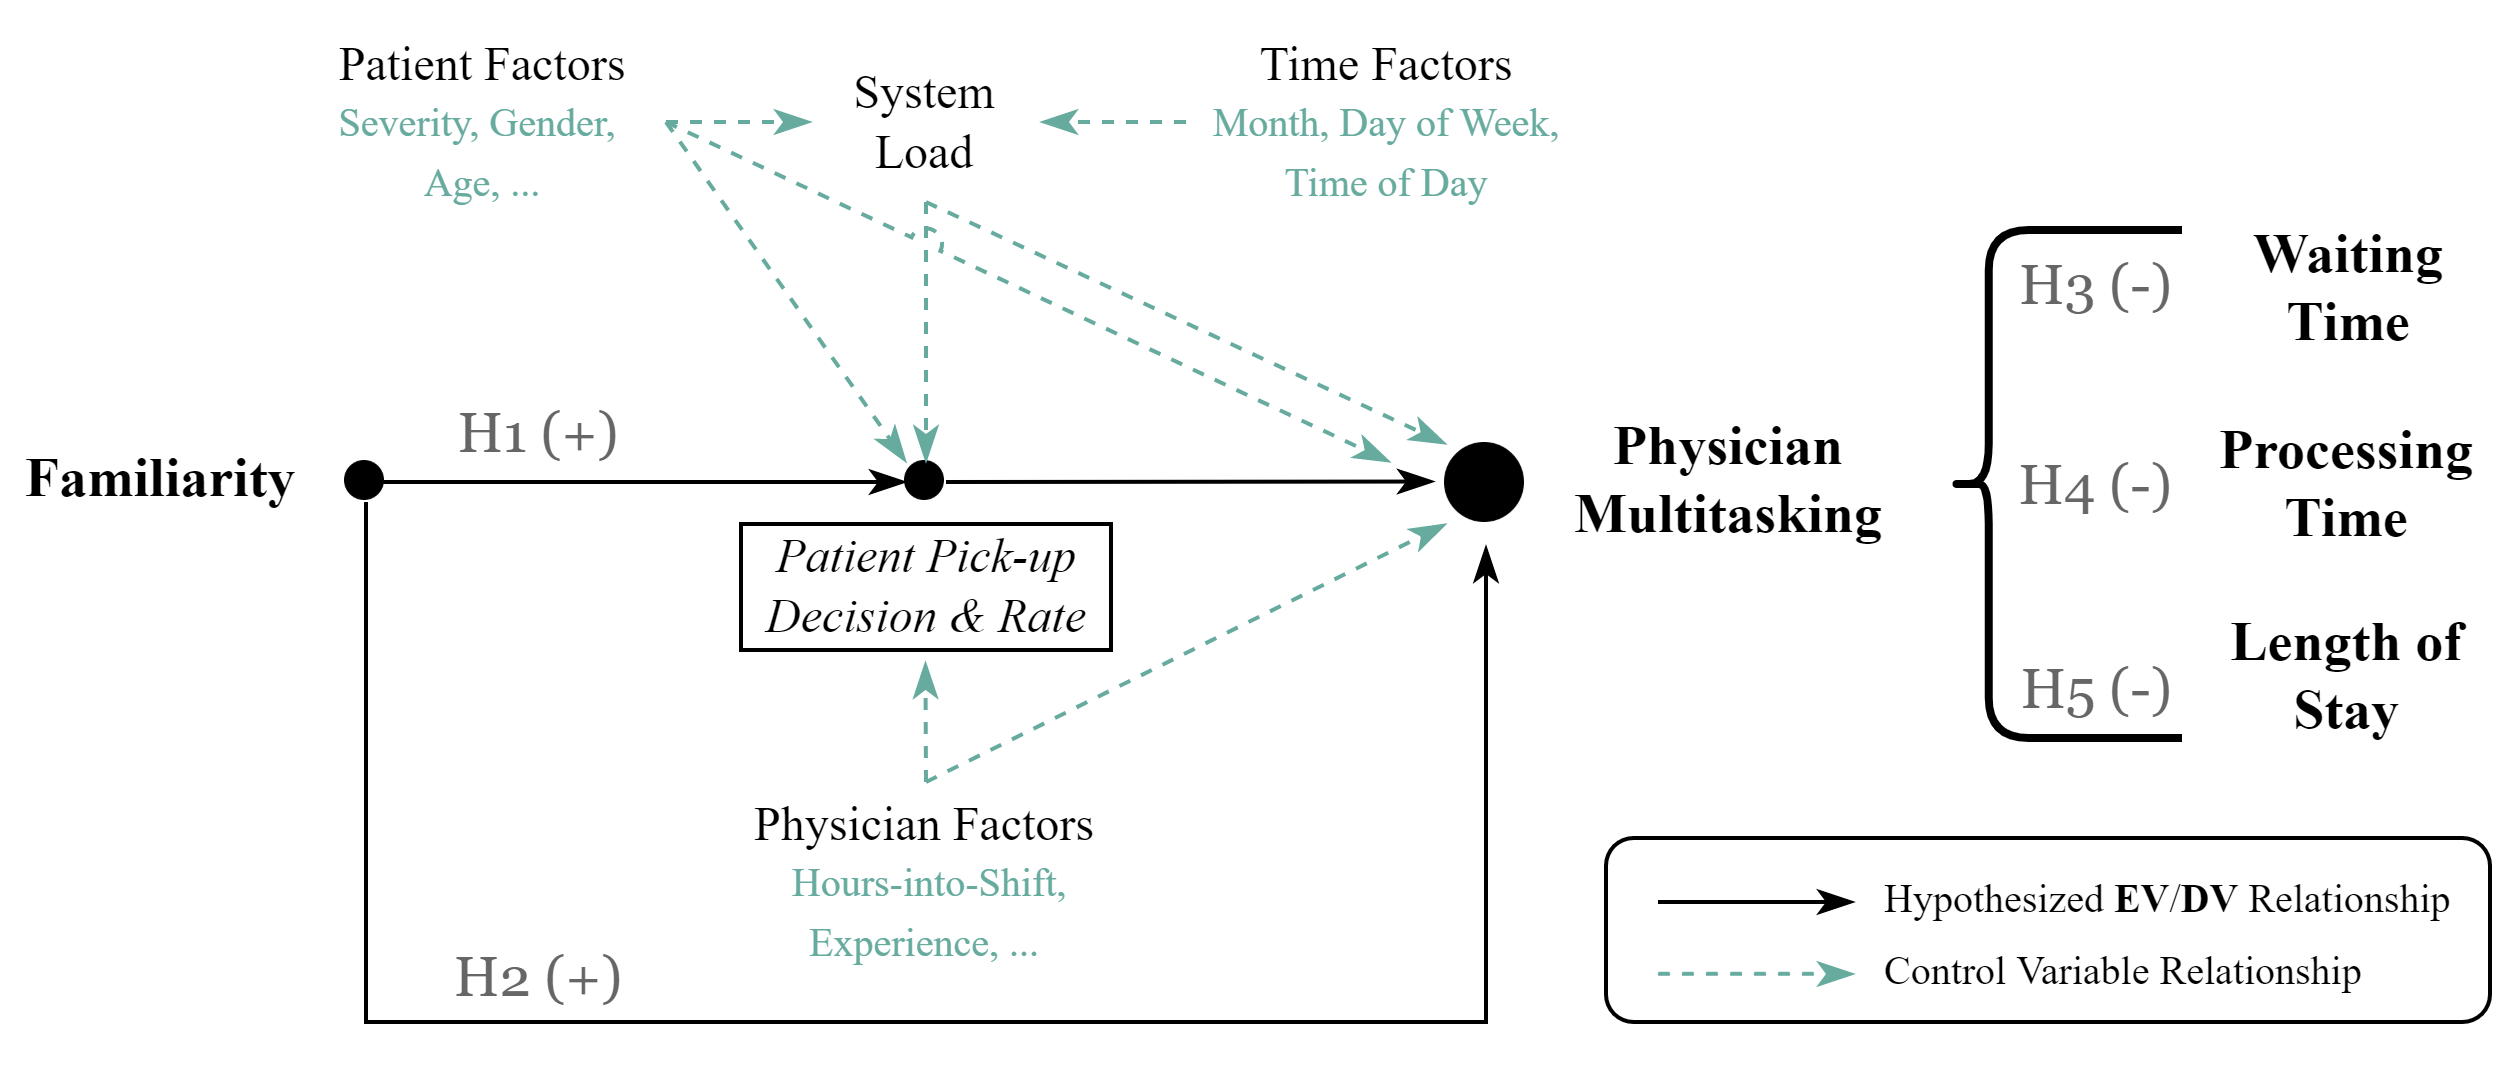
\includegraphics[scale=.8]{Figures/PU/Path Diagram.png}     
     \label{fig:path}
    %  \floatfoot{\textit{Figure Note:} ... some figure notes. }
 \end{figure}
 
 \subsubsection{Familiarity \& Pick-up: A Link to Productivity}
 To start, we consider how systems assign or workers receive tasks. In many contexts, including the ED \citep[see][]{Chan2016}, knowledge workers wield discretion to choose their “work content" \citep[p. 340]{Allon2019}, perhaps through a choice of tasks \citep[e.g.,][]{VanDonselaar2010,KC2020_productivity,Ibanez2017}. We investigate how familiarity affects such task selection in the ED. 
 % While patients are waiting, physician are deciding: “Should I pick up a patient from the queue?"
 
 The ED is an ideal setting for a study of discretion and social exchange: Patients present themselves for treatment, and physicians choose whom to treat. Consider one example from an ED physician: 
 \begin{quote} \textit{At the end of my shift, I might see several straightforward cases and allow another patient with a hazy prognosis to wait an hour. This is because it can actually be \underline{more} beneficial for an ill-defined case to wait, thus avoiding a patient handoff between physicians in the middle of a shift change.} \end{quote} 
 Furthermore, given the prevalence of repeated interactions and the importance of group perceptions, the ED closely resembles the “micro social order" of \cite{Lawler2008}, where “productive exchange bolsters more exchange behavior, more positive feelings, perceptions of cohesion ... and affective attachments to the [group]" (p. 519). Many factors influence the pick-up decision, including patient severity -- see Figure \ref{fig:path} and \cite{Patterson2016} for examples. But after controlling for such factors, we model how familiarity affects the pick-up decision, \textit{ceteris paribus}.
 
 Given such discretion and a social exchange context, familiarity might affect overall productivity through task selection. \cite{Mas2009} find experience working together eliminates the negative effects of social loafing among workers with overlapping shifts (i.e., more familiarity), though too many “unfair exchanges" can harm individual productivity \citep{Kamalahmadi2021}. High group-valence (e.g., groups with friends) further attenuates effort reductions from social loafing \citep{Karau1993}, and friendship among peers can yield greater cooperation \citep{Bandiera2005}. Familiarity has already been linked to productivity, but the channels which facilitate the link remain under-studied.
 
 Our interest lies in the productivity of the group and the performance of the queue. The server who selects and completes more tasks in a fixed amount of time improves both throughput and productivity; the same holds for the physician who picks up and treats more patients. Because familiarity has been shown to improve productivity, to encourage teamwork, and to reduce the tendency to shirk, we expect task pick-up to increase with greater familiarity.
 
 \medskip \noindent
 \begin{tabularx}{\linewidth}{ r X }
    \textbf{Hypothesis 1:} & \textit{An increase in familiarity will lead to an \underline{increase} in the average patient pick-up rate. (H1)} 
 \end{tabularx}   % \medskip
 
 \subsubsection{Familiarity \& Multitasking: An Altered Outcome} 
 Conditional on familiarity altering the pick-up decision, we ask: Does familiarity among physicians influence workload and the decision to multitask? Familiarity affects outcomes such as service rates, and working with friends increases one's capacity to handle extreme loads \citep{Bandiera2010,Hamilton2003}. But whether familiarity affects the decision to multitask remains unanswered. Workload is a well-known input and moderator of productivity in operational settings \citep[e.g.,][]{Schultz1998,Delasay2018}. In our study, we treat workload as one outcome of the patient pick-up decision, and similar to \cite{KC2014}, we define the multitasking load as the number of unique patients actively receiving care from a physician.
 
 The ED is also an ideal setting for a study of familiarity and multitasking behavior \citep[p. 169]{KC2014}: Since patients arrive at different times and visit lengths vary by severity, physicians must simultaneously manage multiple patients by multitasking, perhaps by instructing a nurse to monitor one patient while checking on another. And even though physicians are intrinsically motivated to provide high quality service \citep{Madara2015}, some have told us:
 \begin{quote}\textit{Who I'm working with in the ED matters. If I’m working with a doctor who I don’t know as well, I pay more attention to try to make sure patient pick-ups are equally balanced between us.} \end{quote}
 Hypothesis 1 proposes the pick-up rate will increase with familiarity, but multitasking depends on both pick-up and discharge rate, and so we must examine multitasking separately. In other contexts \citep[e.g.,][]{Aksin2020,Reagans2005,Avgerinos2017}, familiarity increases the rate of \textit{finishing} work, which (in the ED) might imply an increase the rate of discharging patients. The dynamics in the ED are complex, however, and therefore difficult to predict. Physicians manage the queue jointly but, once assigned, work individually. Because familiarity mitigates negative group tendencies surrounding pick-up and enables one to shoulder greater loads, we expect familiarity exerts more influence over patient pick-up than discharge. Under such conditions, greater familiarity would correspond to greater multitasking, and our second hypothesis follows.
% we expect , without meaningfully altering discharge, such that 
% , and so is important to examine individually.  (CITES). The effect is less clear, in this context, since the queue is jointly managed, but once assigned, the work is done individually. As a result, we expect familiarity to mitigate negative group tendencies for pick-up behavior, but not, , thus meaning that  familiarity will correspond to 
 
 \medskip \noindent
 \begin{tabularx}{\linewidth}{ r X }
    \textbf{Hypothesis 2:} & \textit{An increase in familiarity will lead to an increase in physician multitasking. (H2)}
 \end{tabularx}   % \medskip

 \subsubsection{Familiarity \& Patient Time in the ED: The Full Effect}
 Returning to Figure \ref{fig:path}: H1 claims familiarity affects patient pick-up decisions and H2 codifies the effect by demonstrating familiarity changes multitasking behavior. But finding support for these hypotheses immediately invites other questions: Why does the change in behavior matter? Do patients spend less time in the ED as a result? Do physicians work faster? What other factors also change with familiarity and multitasking? We tackle such questions in turn.
 
 Broadly, we explore patient time in the ED, and we consider three sojourn times for a patient: time spent in the waiting room, processing time (or treatment time), and total length of stay (LOS, the sum of waiting and treatment time). Such durations represent common outcomes of interest in healthcare operations \citep[e.g.,][]{KC2009,Song2015,BerryJaeker2017,Batt2017,KC2020_tcp}. Conditional on finding support for H1 and H2, since familiarity encourages physicians to treat more patients simultaneously, we expect patient wait time to decrease with greater familiarity; our third hypothesis follows.  
 
 For processing time, conflicting possibilities emerge. For example, patients benefit from shorter wait time, but what if the physician then picks up too many patients, leading to fatigue and longer length of stay \citep{KC2009,Gans2010,StaatsGino2012}? Conversely, familiarity might lead to more efficient multitasking, which enables a physician to see more patients with a negligible \citep{Maestad2010} or even beneficial \citep{KC2014} impact to patient care. Or, service rate might increase as load increases \citep{Schultz1998} thus lowering overall length of stay \citep{Deo2019}. 
 
 Such discussion eventually converges to an empirical question. Our causal path diagram (Figure \ref{fig:path}) argues familiarity primarily affects the pick-up decision and not the treatment process. Conditional on finding greater multitasking under H2, however, the literature \citep[see][]{Delasay2018} maintains an increase in load (i.e., multitasking in our context) leads to an decrease in processing time, yielding Hypothesis 4. Shorter processing times, combined with shorter wait times (H3), would then imply shorter length of stay, and Hypothesis 5 follows.
 
 \medskip \noindent
 \begin{tabularx}{\linewidth}{ r X }
    \textbf{Hypothesis 3:} & \textit{An increase in familiarity will lead to a \underline{decrease} in patient wait time. (H3)} \\
    \textbf{Hypothesis 4:} & \textit{An increase in familiarity will lead to an \underline{decrease} in patient processing time. (H4)} \\
    \textbf{Hypothesis 5:} & \textit{An increase in familiarity will lead to a \underline{decrease} in patient length of stay. (H5)} \\
 \end{tabularx}    % \medskip 
 

\section{Empirical Setup} \label{Emp_PU}
 \subsection{Data Description}
 Our dataset contains 51,733 observations of Emergency Department physician interactions with a patient who presents themselves to the ED between 1 January and 31 December 2011. In total, we observe 91 unique physicians across the two Emergency Departments of an East-coast hospital. Of these physicians, we observe 81 during January 2011, indicating almost all of our physicians have some prior familiarity with the system and our results are not driven by new physician learning. The dataset contains the patient arrival time to the ED, the time the patient was first seen by a physician, and the time the patient was discharged. Using the timestamps, we can construct the census of the ED at various times as well as the number of patients a physician is currently overseeing. Please see Table \ref{tab:sum_stats} for summary statistics and correlations. After trimming (see Appendix \ref{app_pu_Trim}), we are left with 40,617 observations. 
  
 \begin{table}[htbp]
  \centering
  \caption{Summary Statistics}
  \resizebox{1\textwidth}{!}{
   \begin{threeparttable}
    \begin{tabular}{ccp{20.43em}ccc}
          & \textbf{Variable} & \multicolumn{1}{c}{\textbf{Definition}} & \textbf{Mean} & \textbf{SD} & \textbf{Max} \\
    (1)   & Physician Multitasking Load (count) & Number of patients actively being treated by the focal physician & 4.53  & 2.25  & 14.00 \\
    (2)   & Patient Pick-up Rate (patients per hour) & Number of patients picked up by focal physician per hour of shift & 1.95  & 1.08  & 9.00 \\
    (3)   & Pick Up New Patient (indicator) & Whether a subsequent patient is picked up during the shift of the focal physician & 0.89  & 0.31  & 1.00 \\
    (4)   & Patient Wait Time (min) & Amount of time (in minutes) a patient spends in the system before being seen by physician & 92.21 & 85.01 & 400.00 \\
    (5)   & Patient Length of Stay (min) & Amount of time (in minutes) between patient arrival to  ED and either patient discharge or patient admission to hospital & 378.38 & 227.24 & 1447.00 \\
    (6)   & Average Familiarity (count) & Average of all pairwise familiarity counts for current physician group & 52.12 & 74.51 & 927.00 \\
    (7)   & Group Size, by hour (count) & Number of physicians working in ED during the given hour & 2.40  & 0.53  & 5.00 \\
    \end{tabular}%
    \medskip
    \begin{tablenotes}
      \footnotesize
      \item \textit{Table Note:} For Patient Pick-up Rate, because of data aggregation, the unit of analysis is the hospital-day-hour-provider ($n$ = 23,909). For all other variables the unit of analysis is an individual patient pick-up ($n$ = 40,617). 
    %   \item (*** $p < 0.01$, ** $p < 0.05$, + $p < 0.1$)
    \end{tablenotes}
    \end{threeparttable} } \medskip %
%   \resizebox{.5\textwidth}{!}{ 
%   \begin{tabular}{ccccccc}
%           & (1)   & (2)   & (3)   & (4)   & (5)   & (6) \\
%     (2)   & -0.198 &       &       &       &       &  \\
%     (3)   & 0.020 & 0.039 &       &       &       &  \\
%     (4)   & -0.023 & 0.035 & 0.272 &       &       &  \\
%     (5)   & -0.147 & 0.254 & 0.114 & 0.012 &       &  \\
%     (6)   & 0.100 & 0.020 & 0.054 & -0.024 & 0.047 &  \\
%     (7)   & -0.023 & -0.024 & -0.024 & -0.034 & 0.035 & 0.026 \\
%     \end{tabular} }
  \label{tab:sum_stats}%
 \end{table} %\smallskip

 \subsection{Empirical Context \& Definition of Patient Pick-up} \label{emp_context}
 Figure \ref{fig:ed_flow} illustrates the typical flow of patients through an ED; see \cite{Batt2017} for similar discussion.
 
 \begin{figure}[!b]
     \centering
     \caption{Typical Emergency Department Process Flow } \smallskip
     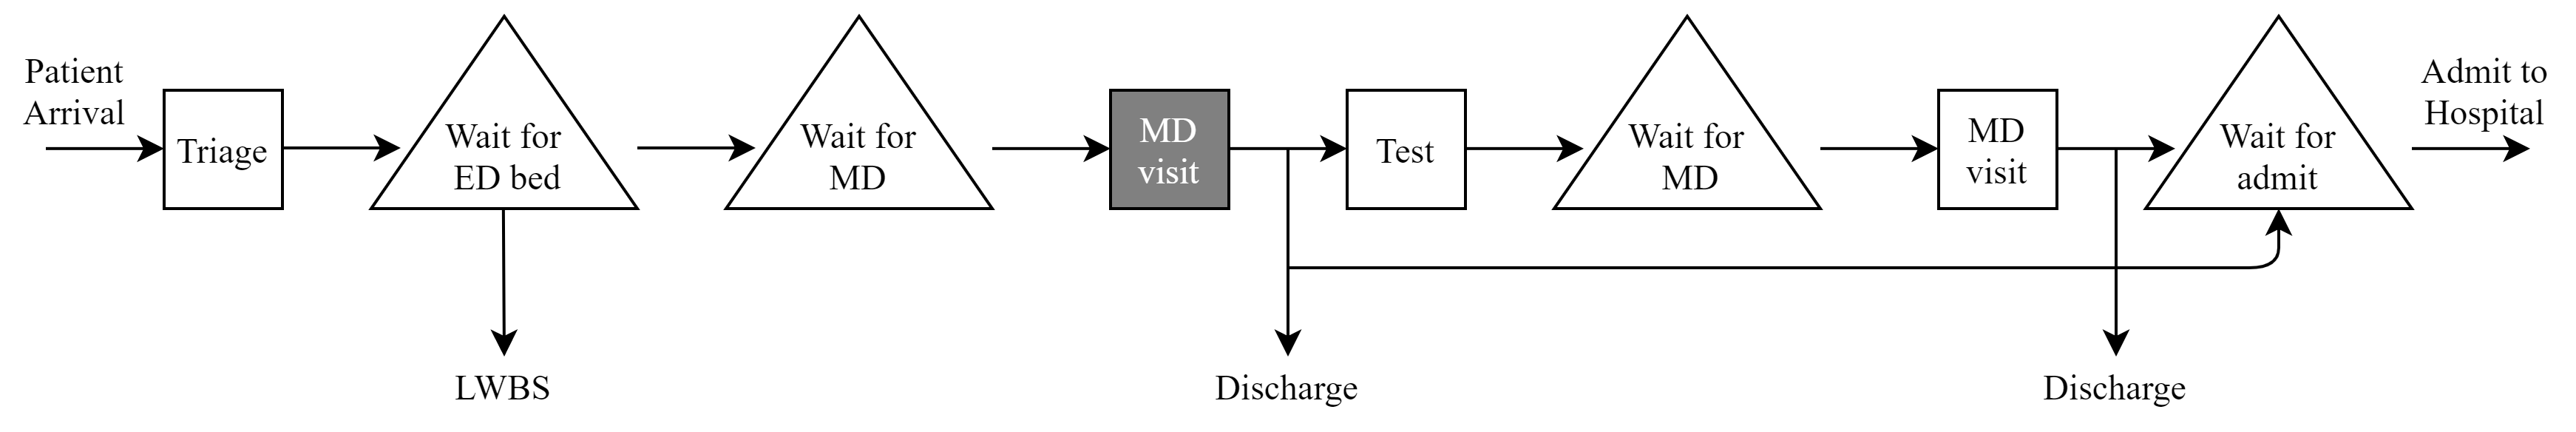
\includegraphics[scale=.7]{Figures/PU/ED Patient Flow-ED Patient Flow.png}     
     \label{fig:ed_flow}
     \floatfoot{\textit{Figure Note:} Patient pick-up occurs with first MD visit (solid gray square). }
 \end{figure}  
 
 For the patient, the process begins with arrival. Upon arriving to the ED, he first interacts with a triage nurse, who assigns each patient a triage acuity level based on the Emergency Severity Index (ESI); triage levels range from 1 to 5 with ESI-1 patients being the most severe patients who should be seen immediately. The nurse also notes the patient’s chief complaint and creates an electronic record for review by the physicians currently on duty. After triage, a patient who chooses to wait then waits until a physician on duty selects to oversee treatment, after which the patient is moved to an ED room and the physician starts treatment. If a patient elects not to wait, he may “leave without being seen” (LWBS), a concept analogous to queue abandonment. In the U.S., national LWBS rates average 1.7\% \citep{Pham2009,Moe2016}, though the rates are further exacerbated by ED crowding \citep{Batt2015}. Although we only consider patients who ultimately encounter a physician, patients who LWBS present an ongoing research problem both in medicine and operations \citep{Saghafian2015,Song2018}. 
 
 For the physician, the process begins with patient selection. Patients are not seen “first-come, first-served" by triage status. Instead the ED record system presents physicians with a list of waiting patients and their status (triage level, chief complaint, etc.). The physician then has discretion to choose who she will treat. For the purposes of our paper, \textit{patient pick-up} occurs when the physician first visits the patient (the solid gray square in Figure \ref{fig:ed_flow}). The physician then oversees care until the patient is discharged, admitted to the hospital, or the physician finishes her shift. At the end of a shift, a physician transfers the care of all remaining patients to another physician through patient “handoffs” \citep[for discussion, see][]{Batt2019}. Thus, a group of physicians enable the smooth handling of operations in an ED, and we proceed by considering the “groups” more critically.

 \subsection{Group Construction} \label{grp_con}
 We first consider how to define an ED “group” or team. ED physicians generally work 8-hour shifts, but the shifts are not rigid. Depending on the ED occupancy and the severity of patients currently waiting, many physicians may extend a shift beyond the required 8 hours. Our dataset groups a given physician’s shift by patient seen during the shift, but it does not indicate when physicians first reported on duty or when they ultimately left the ED; it only contains the observations of the physician selecting patients. Using such information, we can identify each patient seen, and particularly identify the last patient seen during a physician’s shift.
 
 To define an ED physician group, we first bin the dataset observations by hour-of-day. A physician belongs to the hour’s group if and only if the physician is observed picking up a patient during that hour. Such an approach conservatively avoids documenting familiarity when we cannot be certain the physicians were actively working together. Since we are interested in the outcomes from interactions between physicians, following \cite{Avgerinos2017}, we define a pair of group members as the smallest subset of a group. Individual pairs form our units of analysis as we explore how differing experience between pairs in the same group impacts our outcome variables. Since we are interested in the impact of familiarity on patient pick-up behavior, we count each patient pick-up as one additional instance of pairwise familiarity. Such a construction measures the cumulative quantity of task decisions within a group. Our conclusions are also robust to analyzing the cumulative volume of time spent together, where each hour spent working overlapping shifts is counted as an additional instance of pairwise familiarity. Please see the Appendix \ref{app_pu_examples} for an example panel which illustrates group construction and the incrementing of pairwise familiarity measures.

 \subsection{Dependent Variables} \label{emp_DV}
 We explore the impact of familiarity on several outcome measures. To start, we propose familiarity affects the patient pick-up decisions of physicians and we consider such decisions the means by which familiarity might affect other ED outcomes. To test our proposition, we implement two operationalizations of the patient pick-up decision and the resulting pick-up rate (H1). First, to measure the ED flow rate, we aggregate our data to the hourly level and measure the rate in patient pick-ups per hour. But because of the required aggregation, such an outcome cannot consider patient heterogeneity (e.g., patient severity, age, etc.) as an input. As a supplemental approach which does not ignore patient heterogeneity, we also model the pick-up decision as the likelihood of a physician picking up one additional patient. During a given shift, a binary indicator variable takes the value 1 if another patient is selected after the current observation, and the indicator switches to zero for the last patient of a physician's shift. Though we do not observe when shifts end, in effect the indicator variable captures that a physician has decided to stop working sometime after the last patient pick-up of the shift. Please see Appendix \ref{app_pu_examples} for an illustrative example of our indicator variable.

 Assuming we find familiarity affects the pick-up decision, we can then explore if familiarity affects other ED outcomes. We proceed by exploring how familiarity affects multitasking, measured as the number of patients actively being treated by a physician (H2). Our study concludes by determining the effect of familiarity on different patient visit durations: Wait time (H3), processing time (H4), and length of stay (H5).
 
 \subsection{Explanatory Variable}
 Formally, we define \textit{average familiarity} for the physician $i$ in physician-group $G$ composed of physician-pairs $p$ during the current hour $h$ which contains the patient pick-up which occurs at time $t$ (day-hour-minute):
 \begin{equation} \label{eq_fam}
     AverageFamiliarity_{it} = \frac{ \sum_{p \in G_h} \sum_{s=1}^t Joint\_PickUp_{ps} }{ N_h * (N_h-1)/2 }
 \end{equation}
 \noindent 
 Specifically, we take the following steps. First, we consider each hour $h$ in our data. Second, we note all physicians who pick up a patient within the hour; such physicians represent the hour’s physician group ($G_h$, see Section \ref{grp_con}). Third, we cumulatively sum all previous pairwise familiarity ($Joint\_PickUp$) for each physician pair $p$ in the group for patient pick-ups from the start of the data ($s=1$) up to time $t$. Fourth, we sum the pairwise familiarities for all physician pairs in the group ($p \in G_h$). Fifth, in line with literature on average familiarity, we divide the sum of pairwise familiarities for all group pairs by $N_h*(N_h-1)/2$, where $N_h$ represents size of group $G_h$ during hour $h$. Please see Appendix \ref{app_pu_examples} for an example panel which illustrates the construction of our variables in a hypothetical panel. As in previous literature \citep[e.g.,][]{Avgerinos2017}, we log-transform average familiarity and only consider familiarity gained prior to the current patient pick-up in our models in Section \ref{em_spec}.

 \subsection{Control Variables} \label{ctrl_vars}
 Building on the proposed causal paths and the important factors illustrated in Figure \ref{fig:path}, we include the following control variables to mitigate concerns of confounding. In our probit model of pick-up likelihood (Section \ref{spec_probit}), in line with Chamberlain’s random effects probit model, we also include a Mundlak device ($\bar{X_i}$) – the individual averaged values of all control variables.
 
 \noindent \textbf{Physician Controls.} We control for an individual physician fixed effect, physician hours-into-shift, the number of physicians in the current group, and physician experience. Such a measure controls for any learning which correlates with familiarity by counting the cumulative number of patients picked up during our study; see Appendix \ref{app_pu_examples} for examples. Similar to \cite{Reagans2005}, we log-transform experience and also include experience squared, to capture any diminishing returns of experience. 
 
 \noindent \textbf{Patient Controls.} We control for patient gender, an indicator for patients older than 65, patient triage level, and patient arrival factors: Time of day (Morning: 7a-3p, Afternoon: 3p-11p, Overnight: 11p-7a), day of week, and month. 
 
 \noindent \textbf{ED Controls.} We include a fixed effect for each ED and three separate measures of ED load: (i) individual physician load, (ii) the sum of the physician loads across the current group, and (iii) waiting room census. Such characteristics might affect patient pick-up decisions. To avoid including “bad controls” , or variables which are themselves potential outcome variables, we use lagged versions of the variables since they are “measured before the variable of interest (i.e., patient pick-up) was determined" \citep[p. 68]{Angrist2009}. Variables determined in the past cannot possibly represent future outcomes, and so our approach mitigates such concerns.

 \subsection{Threats to Identification}
 We maintain our explanatory variables for familiarity serve as valid independent variables for the following reasons. First and foremost, physician ED scheduling is generally controlled by a master scheduler with whom the scheduling decisions rests. The scheduler does not consider physician familiarity as an important factor. Furthermore, we also include multiple time fixed effects as control variables (time of day, day of week, and month). As such, our models absorb any preference -- such as a preference for the night shift or to work with a familiar colleague -- which correlates with the fixed effects. Any residual effect can thus be attributed to physician familiarity, and so we treat our familiarity variable as exogenous. Second, because physicians largely treat patients separate from other physicians, we see little reason for physicians to synchronize schedules with another physician. Examining our data shows there are no pairs who only work with one another, consistent with such a synchronization approach. Third, we imitate similar studies of familiarity; the approach of the literature focuses on familiarity gained before the current observation, providing temporal separation between familiarity and immediate patient pick-up. Fourth, because of the richness of our data, we include many control variables, mitigating concerns of omitted variable bias while also controlling for possible temporal correlation. Finally, our results are robust and consistent across several model specifications, each of which requires varying levels of independence. Most notably, accelerated-failure-time models are robust even in the presence of omitted variables \citep{Keiding1997}. Based on the arguments above, we conclude our variables represent sufficiently exogenous measures to proceed.
 
 \subsection{Econometric Specifications} \label{em_spec}
 We apply three different econometric approaches to evaluate our outcomes: A linear fixed effect framework \citep[Ch. 10]{Wooldridge2010}, a random effects probit model \citep[Ch. 15]{Wooldridge2010}, and a duration (or hazard) regression framework \citep{Cleves2016}. We refer interested readers to \cite{Batt2017} and \cite{Batt2019} for other examples of duration models in operations research. 
 
 In addition to our primary explanatory variable ($AverageFamiliarity_{it}$), we define the following variables for physician $i$ at time $t$: $HIS_{it}$ represents hours worked during the shift; $Exp_{it}$ captures physician experience; $GroupSize_t$ captures the current physician group size; $Occ^{Wait}$ captures the waiting room occupancy; $Occ^{Treat}$ captures the number of patients currently receiving treatment; and $Hosp_i$ represents a hospital specific fixed effect. Additionally, $c_i$ represents the unobservable physician specific effects, $\boldsymbol{\delta_t}$ represents a vector of time varying controls (month, day of week, and time of day), and $\boldsymbol{\theta_t}$ represents a vector of patient varying controls (gender, age, and triage status).
 
 \subsubsection{Linear Fixed Effect Models (H1, H2)} \label{spec_linear}
 Hypothesis 1 and Hypothesis 2 evaluate the effect of average familiarity on two outcomes: pick-up rate and physician multitasking, for physician $i$ during the patient pick-up at time $t$ (day-hour-minute). In the regressions, we cluster the errors at the physician level to correct for serial correlation and heteroskedasticity within physicians, in-line with the discussion of clustering in \cite{Bertrand2004}. 
 
 As a first evaluation of \textbf{pick-up rate} (H1), we start with an outcome variable ($PickupRate_{it}$) which captures the the total number of patients physician $i$ picks up during time-interval $t$. To assess the hourly rate, we aggregate the data to the hospital-day-hour-physician level. We choose to aggregate our remaining variables by selecting the \textit{maximum} observed value during hour $t$; such a choice captures the state of the system at (a) the end of the hour, or (b) its most congested point. Thus, in the following specification for physician $i$ during hour $t$ (day-hour), $\ddot{\ln(AverageFamiliarity_{it})}$ represents the maximum of $\ln(AverageFamiliarity_{it})$ during hour $t$, $\ddot{\ln (Exp_{it})}$ represents the maximum of $\ln(Exp_{it})$, $\ddot{Occ}^{Wait}$ represents the maximum of $Occ^{Wait}$, $\ddot{Occ}^{Treat}$ represents the maximum of $Occ^{Treat}$, and $\epsilon_{it}$ captures any remaining idiosyncratic shocks. All other variables remain the same as defined above, though the aggregation process drops patient specific variables (i.e., $\boldsymbol{\theta_t}$).
  \begin{equation} \label{eqn_pu_rate_1} \begin{split} %
       PickupRate_{it} = \gamma_0 & + \gamma_1 \ddot{\ln(AverageFamiliarity_{it})} +  HIS_{it} + \ddot{\ln (Exp_{it})} + [\ddot{\ln (Exp_{it})}]^2 \\
       & + GroupSize_{t} + \ddot{Occ}_{t-1}^{Wait} + \ddot{Occ}_{t-1}^{Treat} \\
       & + Hosp_i + c_i + \boldsymbol{\delta_t} + \epsilon_{it} 
  \end{split}  \end{equation}
 
 To evaluate \textbf{multitasking} (H2), we start with an outcome variable ($PhysMultitasking_{it}$) which captures the number of patients actively being treated by physician $i$ at time $t$ (day-hour-minute). The specification includes the control variables defined above, and $\epsilon_{it}$ captures any remaining idiosyncratic shocks.
  \begin{equation} \begin{split} %
       PhysMultitasking_{it} = \alpha_0 & + \alpha_1 \ln(AverageFamiliarity_{it}) + HIS_{it} + \ln(Exp_{it}) + [\ln(Exp_{it})]^2 \\
       & + GroupSize_{t} + Occ_{t-1}^{Wait} + Occ_{t-1}^{Treat} \\
       & + Hosp_i + c_i + \boldsymbol{\delta_t} + \boldsymbol{\theta_t} + \epsilon_{it} 
  \end{split}  \end{equation}
  
 \subsubsection{Random Effects Probit Model (H1)} \label{spec_probit}
 As discussed in Section \ref{emp_DV} for Hypothesis 1, we also apply a second model to measure patient \textbf{pick-up rate} which includes patient heterogeneity and does not drop patient specific variables (i.e., $\boldsymbol{\theta_t}$). Using the Probit link function, our approach models the likelihood of physician $i$ picking up another patient \textit{after} the observed pick-up at time $t$ (day-hour-minute). We implement Chamberlain’s random effects probit model, evaluated via pooled maximum likelihood estimation \citep[Ch. 15]{Wooldridge2010}, where $\boldsymbol{\Phi}$ represents the Normal cumulative distribution function and $\eta_{it}$ represents our idiosyncratic error. To further refine the precision of our estimates, the specification can also include a variable which controls for the prior physician multitasking level ($PhysMultitasking_{i,t-1}$). To further ensure model validity: (i) We control for serial time dependence by clustering our errors at the physician level; and (ii) we include a Mundlak device ($\boldsymbol{\bar{X_i}}$), which relaxes an assumption and allows other variables to be correlated with $c_i$.
  \begin{equation} \label{eqn_pu_rate_2} \begin{split} %
        \text{Prob} (PatientPickup_{it}) = \boldsymbol{\Phi} (\pi_0 & + \pi_1 \ln(AverageFamiliarity_{it}) + HIS_{it} + \ln(Exp_{it}) + [\ln(Exp_{it})]^2 \\
       & + GroupSize_{t} + Occ_{t-1}^{Wait} + Occ_{t-1}^{Treat} + PhysMultitasking_{i,t-1} \\
       & + \boldsymbol{\bar{X_i}} + Hosp_i + c_i + \boldsymbol{\delta_t} + \boldsymbol{\theta_t} + \eta_{it} )
  \end{split}  \end{equation}

 \subsubsection{Duration Regression Model (H3, H4, H5)} \label{spec_hazard}
 Hypotheses 3, 4, and 5 evaluate the impact of familiarity on three durations: The time spent waiting to see a physician (H3), the time to finish treatment on a patient once started (H4), and the total amount of time a patient spends in the ED, or length of stay (H5). As such, we apply an accelerated-failure-time (AFT) model, a form of parametric duration (or hazard) regression. Such a model evaluates the duration or time-to-failure, where the baseline hazard is allowed to vary over time with the covariates as above, which also vary over time:
  \begin{equation}
  h(t|\boldsymbol{X_{it}}) = h_0(t) \exp(\boldsymbol{X_{it}} \boldsymbol{\beta})
  \end{equation}
 
 In our case, “time to failure” is “time to pick-up.” Such a form models the relationship of a linear combination of covariates to different durations for the patient visit at time $t$ (day-hour-minute) who is treated by physician $i$. We maintain a highly flexible specification in assuming a generalized gamma distribution for the model, and such a distribution also provides the best model fit based on the Akaike and Bayesian Information Criteria. We specify our linear combination of covariates as follows. We also stratify by ED, allowing the shape and scale of the hazard function to vary for each ED. In the regressions, we cluster the errors at the time of day level, for each day in our dataset, to correct for serial correlation and heteroskedasticity within clinics, in-line with the discussion of clustering in Chapter 10 of \cite{Cleves2016}. Our approach to modeling patient time in the ED closely mirrors the approach of \cite{Batt2017}.
  \begin{equation} \begin{split} %
        \boldsymbol{X_{it}}\boldsymbol{\beta} = (1 & + \ln(AverageFamiliarity_{it}) + HIS_{it} + \ln(Exp_{it}) + [\ln(Exp_{it})]^2 \\
        & + GroupSize_t + Occ_{t-1}^{Wait} + Occ_{t-1}^{Treat}   \\
        & + Hosp_i + c_i + \boldsymbol{\delta_t} + \boldsymbol{\theta_t} ) * \boldsymbol{\beta}
  \end{split}  \end{equation}
  % + PhysMultitasking_{i,t-1}
  
  
\section{Results} \label{Results_PU}
 \subsection{H1: Familiarity \& Patient Pick-up} \label{results_H1}
 To start, we seek to answer the question: Does familiarity affect patient pick-up? We propose the task selection decision (i.e., patient pick-up) provides a channel through which familiarity can affect other ED outcomes, such as multitasking. When patients are waiting in the waiting room and a physician has spare capacity, a physician faces a choice: (a) “Should I pick up another patient?" or (b) “Should I forgo this opportunity and focus on my current patients, leaving waiting patients for later or for another physician?" We model the effect of familiarity on such a decision in two ways: First, by considering whether familiarity increases an aggregate measure of ED flow rate (measured in patients per hour), and second, by considering whether familiarity increases the \textit{likelihood} of (a) while still considering patient heterogeneity as an input. Table \ref{tab:pu_H1H2}, Columns (1) and (2) present the results; full regression results can also be found in Appendix \ref{pu_full_reg}. 
  % Or, in other words, what is the intermediate action by which familiarity might affect other ED outcomes, such as multitasking?
 % Our previous finding provokes the following question: How does familiarity increase physician multitasking? 
 
 In the first case, we do see an increase in average familiarity corresponds to an increase in pick-up rate, and the effect is statistically significant ($p < 0.01$). A 1\% increase in familiarity corresponds to an increase of 0.0319 patient pick-ups per hour. Relative to the median pick-up rate of 2 patients per hour, the increase corresponds to a 1.6\% increase in pick-up rate. Furthermore, we also see familiarity has a positive and statistically significant ($p < 0.01$) impact on the likelihood of a physician picking up one additional patient. The Average Partial Effect (APE) shows a 1\% increase in average familiarity corresponds to a 1.04\% increase in the patient pick-up likelihood. Together, both findings provide congruous support for Hypothesis 1: Greater average familiarity increases the patient pick-up rate of physicians.
 
 As a check for consistency, Appendix \ref{app_pu_hazard_between} presents an alternative to modeling patient pick-up rate (specifications (\ref{eqn_pu_rate_1}) and (\ref{eqn_pu_rate_2})) by modeling the effect of familiarity on the time between patient pick-ups for a physician. Our conclusions hold here, as the results show an increase in familiarity also reduces the time between pick-ups ($p < 0.01$).
 
 \subsection{H2: Familiarity \& Multitasking}
 Since we have shown familiarity does affect the patient pick-up decision, we then consider the effect of familiarity on physician multitasking levels. Table \ref{tab:pu_H1H2}, Column (3) reports the results of the model. We see familiarity has a positive and statistically significant ($p < 0.01$) effect on physician multitasking. The Average Partial Effect shows a 1\% increase in average familiarity leads to an increase in physician multitasking by 0.141 patients. That is, when a physician is working with more familiar peers, she increases her patient load, or the number of patients she is willing to treat at any given time. Relative to the median physician multitasking load of 4 patients, the effect corresponds to a 3.5\% increase in physician multitasking. The finding supports Hypothesis 2: Greater average familiarity increases physician multitasking in the ED.
 
\begin{table}[htbp]
  \resizebox{.9\textwidth}{!}{ 
  \begin{threeparttable}[t]
   \centering
   \caption{More familiarity increases  the rate of patient pick-up and physician multitasking.}
    \begin{tabular}{lcccc}
          & (1)   & \multicolumn{2}{c}{(2)} & (3) \\
    Output Variable & \textbf{Pick-up Rate} & \multicolumn{2}{c}{\textbf{Pick-up Likelihood}} & \textbf{Multitasking} \\
    Hypothesis & H1    & \multicolumn{2}{c}{H1} & H2 \\
    Model & Linear FE & \multicolumn{2}{c}{Chamberlain RE Probit} & Linear FE \\
    Estimation Method & Coefficient/APE & Coefficient & APE   & Coefficient/APE \\
          &       &       &       &  \\
    \textit{Average Familiarity} & 0.0319*** & 0.0959*** & 0.0104*** & 0.141*** \\
          & (0.00796) & (0.0134) & (0.00146) & (0.0168) \\
    \textit{Waiting Room Occupancy} & 0.0452*** & -0.0117*** & \textcolor[rgb]{ .749,  .749,  .749}{-} & 0.000254 \\
          & (0.00302) & (0.00395) & \textcolor[rgb]{ .749,  .749,  .749}{-} & (0.00435) \\
    \textit{ED Seen Occupancy} & 0.0154*** & 0.0575*** & \textcolor[rgb]{ .749,  .749,  .749}{-} & 0.145*** \\
          & (0.00183) & (0.00424) & \textcolor[rgb]{ .749,  .749,  .749}{-} & (0.00507) \\
    \textit{Physician Hours into Shift} & -0.200*** & -0.619*** & \textcolor[rgb]{ .749,  .749,  .749}{-} & 0.634*** \\
          & (0.00607) & (0.0247) & \textcolor[rgb]{ .749,  .749,  .749}{-} & (0.00991) \\
    \textit{Physician Experience (linear)} & 0.0382 & 0.130 & \textcolor[rgb]{ .749,  .749,  .749}{-} & 0.380*** \\
          & (0.0414) & (0.115) & \textcolor[rgb]{ .749,  .749,  .749}{-} & (0.0755) \\
    \textit{Physician Experience (quadratic)} & 0.00364 & -0.0112 & \textcolor[rgb]{ .749,  .749,  .749}{-} & -0.0468*** \\
          & (0.00589) & (0.0133) & \textcolor[rgb]{ .749,  .749,  .749}{-} & (0.0121) \\
          &       &       &       &  \\
    Physician Controls: Group Size, Phys. FE & Y     & \multicolumn{2}{c}{Y} & Y \\
    Patient Controls: Age, Gender, Severity & N     & \multicolumn{2}{c}{Y} & Y \\
    ED Controls: Hosp. FE, ToD, DoW, Month & Y     & \multicolumn{2}{c}{Y} & Y \\
          &       &       &       &  \\
    Physicians & 91    & \multicolumn{2}{c}{91} & 91 \\
    Observations & 23,909 & \multicolumn{2}{c}{40,617} &  40,617  \\
    \end{tabular}%
    \medskip
    \begin{tablenotes}
      \footnotesize
      \item \textbf{Table Note:} Robust standard errors clustered at the physician level reported in parentheses. Models include controls listed in Section \ref{em_spec}. Pick-up Rate measured in patient pick-ups per hour. Results reported in Column (1) aggregate observations to the hourly level, thus omitting patient specific characteristics as discussed in Section \ref{spec_linear}. Abbreviations: APE (Average Partial Effect), Phys. (Physician), FE (Fixed Effect), Hosp. (Hospital), ToD (Time of Day), DoW (Day of Week). (*** $p < 0.01$, ** $p < 0.05$, + $p < 0.1$)
    %   \item (*** $p < 0.01$, ** $p < 0.05$, + $p < 0.1$)
    \end{tablenotes}
  \label{tab:pu_H1H2}
  \end{threeparttable} }
 \end{table}
 
\begin{table}[htbp]
  \resizebox{1\textwidth}{!}{ 
  \begin{threeparttable}[t]
   \centering
   \caption{More familiarity decreases patient wait time, but does not affect processing time or length of stay.}
    \begin{tabular}{lcccccc}
          & \multicolumn{2}{c}{(1)} & \multicolumn{2}{c}{(2)} & \multicolumn{2}{c}{(3)} \\
    Output Variable & \multicolumn{2}{c}{\textbf{Wait Time}} & \multicolumn{2}{c}{\textbf{Processing Time}} & \multicolumn{2}{c}{\textbf{Length of Stay}} \\
    Hypothesis & \multicolumn{2}{c}{H3} & \multicolumn{2}{c}{H4} & \multicolumn{2}{c}{H5} \\
    Model & \multicolumn{2}{c}{AFT Duration} & \multicolumn{2}{c}{AFT Duration} & \multicolumn{2}{c}{AFT Duration} \\
    Estimation Method & Coefficient & APE (min) & Coefficient & APE (min) & Coefficient & APE (min) \\
          &       &       &       &       &       &  \\
    \textit{Average Familiarity} & -0.0155** & -1.172** & -0.0000725 & -0.017 & -0.00330 & -1.101 \\
          & (0.00646) & (0.489) & (0.00392) & (0.929) & (0.00325) & (1.083) \\
    \textit{Waiting Room Occupancy} & 0.0931*** & \textcolor[rgb]{ .749,  .749,  .749}{-} & -0.00577*** & \textcolor[rgb]{ .749,  .749,  .749}{-} & 0.0237*** & \textcolor[rgb]{ .749,  .749,  .749}{-} \\
          & (0.00213) & \textcolor[rgb]{ .749,  .749,  .749}{-} & (0.00105) & \textcolor[rgb]{ .749,  .749,  .749}{-} & (0.000873) & \textcolor[rgb]{ .749,  .749,  .749}{-} \\
    \textit{ED Seen Occupancy} & 0.0129*** & \textcolor[rgb]{ .749,  .749,  .749}{-} & 0.00567*** & \textcolor[rgb]{ .749,  .749,  .749}{-} & 0.00705*** & \textcolor[rgb]{ .749,  .749,  .749}{-} \\
          & (0.00163) & \textcolor[rgb]{ .749,  .749,  .749}{-} & (0.000875) & \textcolor[rgb]{ .749,  .749,  .749}{-} & (0.000750) & \textcolor[rgb]{ .749,  .749,  .749}{-} \\
    \textit{Physician Hours into Shift} & -0.00153 & \textcolor[rgb]{ .749,  .749,  .749}{-} & -0.0225*** & \textcolor[rgb]{ .749,  .749,  .749}{-} & -0.0146*** & \textcolor[rgb]{ .749,  .749,  .749}{-} \\
          & (0.00240) & \textcolor[rgb]{ .749,  .749,  .749}{-} & (0.00170) & \textcolor[rgb]{ .749,  .749,  .749}{-} & (0.00125) & \textcolor[rgb]{ .749,  .749,  .749}{-} \\
    \textit{Physician Experience (linear)} & 0.122*** & \textcolor[rgb]{ .749,  .749,  .749}{-} & 0.0729*** & \textcolor[rgb]{ .749,  .749,  .749}{-} & 0.0829*** & \textcolor[rgb]{ .749,  .749,  .749}{-} \\
          & (0.0304) & \textcolor[rgb]{ .749,  .749,  .749}{-} & (0.0186) & \textcolor[rgb]{ .749,  .749,  .749}{-} & (0.0161) & \textcolor[rgb]{ .749,  .749,  .749}{-} \\
    \textit{Physician Experience (quadratic)} & -0.0142*** & \textcolor[rgb]{ .749,  .749,  .749}{-} & -0.00744*** & \textcolor[rgb]{ .749,  .749,  .749}{-} & -0.00871*** & \textcolor[rgb]{ .749,  .749,  .749}{-} \\
          & (0.00464) & \textcolor[rgb]{ .749,  .749,  .749}{-} & (0.00283) & \textcolor[rgb]{ .749,  .749,  .749}{-} & (0.00245) & \textcolor[rgb]{ .749,  .749,  .749}{-} \\
          &       &       &       &       &       &  \\
    Physician Controls: Group Size, Phys. FE & \multicolumn{2}{c}{Y} & \multicolumn{2}{c}{Y} & \multicolumn{2}{c}{Y} \\
    Patient Controls: Age, Gender, Severity & \multicolumn{2}{c}{Y} & \multicolumn{2}{c}{Y} & \multicolumn{2}{c}{Y} \\
    ED Controls: Hosp. FE, ToD, DoW, Month & \multicolumn{2}{c}{Y} & \multicolumn{2}{c}{Y} & \multicolumn{2}{c}{Y} \\
          &       &       &       &       &       &  \\
    Physicians & \multicolumn{2}{c}{91} & \multicolumn{2}{c}{91} & \multicolumn{2}{c}{91} \\
    Observations & \multicolumn{2}{c}{                           40,617 } & \multicolumn{2}{c}{                             40,617 } & \multicolumn{2}{c}{                             40,617 } \\
    \end{tabular}%
    \medskip
    \begin{tablenotes}
      \footnotesize
      \item \textbf{Table Note:} Accelerated Failure Time (AFT) duration models include robust standard errors (reported in parentheses) which are clustered at the time of day level for each day in our dataset. Models include controls listed in Section \ref{em_spec}. Abbreviations: APE (Average Partial Effect), Phys. (Physician), FE (Fixed Effect), Hosp. (Hospital), ToD (Time of Day), DoW (Day of Week).  (*** $p < 0.01$, ** $p < 0.05$, + $p < 0.1$)
    %   \item (*** $p < 0.01$, ** $p < 0.05$, + $p < 0.1$)
    \end{tablenotes}
  \label{tab:H3H5}
  \end{threeparttable} }
 \end{table}

 \subsection{H3-H5: Familiarity \& Time in the ED}
 Our previous results demonstrate (i) familiarity affects the patient pick-up decision (H1), and (ii) familiarity increases physician multitasking (H2). Nevertheless, because our empirical setting is an actual ED and not a laboratory, we cannot claim with full certainty that the pick-up decision serves as the only link between familiarity and multitasking. And yet, if our causal paths proposed in Figure \ref{fig:path} can withstand some sensitivity analysis, then we can be even more confident in the validity of our model. Additionally, beyond simply establishing a link, we seek to inform decision makers and policy outcomes. We proceed to discuss other implications for ED operations generated by our causal model and previous findings.
 
 Next, we consider the time a patient spends in the ED, and we separate it out into time spent waiting, patient processing time, and total length of stay. Table \ref{tab:H3H5} presents the results of the regressions; the table reports the Average Partial Effects of the duration regression models in minutes. From the table, we observe an increase in familiarity does correspond to a decrease in patient wait time, and the result is statistically significant ($p < 0.05$). The Average Partial Effect shows a 1\% increase in average familiarity corresponds to a 1.172-minute decrease in patient waiting time, or a 1.9\% decrease relative to the median waiting time of 62 minutes. The finding supports Hypothesis 3: Greater average familiarity reduces the time patients spend waiting to see a physician. And yet we cannot reject the null hypothesis that familiarity has no impact on patient processing time or length of stay. Thus, we find no evidence here to support Hypothesis 4 or Hypothesis 5. One possible explanation: Since familiarity leads to more multitasking, and since high levels of multitasking can negatively affect service rate \citep[e.g.,][]{KC2014}, perhaps we observe a null effect on patient processing time because of a “net" effect of familiarity. The following section concludes with a general discussion of our results and a post-hoc analysis.
 
 \subsection{Summary \& Post-hoc Analysis}
 To determine the effect of familiarity on physician productivity, we started by suggesting one channel through which familiarity may influence the decision to multitask. We hypothesized greater average familiarity increases the patient pick-up rate of physicians, which then leads to more physician multitasking. In other words, familiarity increases the willingness of a physician to treat more patients simultaneously, which then manifests in decisions to pick-up more patients.
 
 Indeed, we found this to be true. But then we wonder: Might the pick-up rate increase more for some portion of a shift? \cite{Ouyang2021} demonstrate the importance of considering “... shift-hour-dependent service rates in ED modeling and staffing" (p. 25). \cite{Deo2019} find an increase in service rate among clinicians at the end of the workday while \cite{Chan2018} finds some physicians “slack off" at the end of a shift. At the end of a shift the physician must choose: “Do I continue working and pick up more patients, or if I have finished my shift, do I go home?” Although all patients who do not leave without being seen are eventually picked up, organizational factors (e.g., shift changes), human behavior, and physician discretion collide at just this point in time. As such, we propose some effects of familiarity might intensify at the end of the shift.
 
 In our context, we focus on the last observed hour of a shift for each physician, which \cite{Ouyang2021} refers to as the “end-of-shift phase." We do find familiarity increases the patient pick-up rate even more during this window. A 1\% increase in familiarity corresponds to an increase of 0.0691 patient pick-ups per hour during the last observed hour of the shift ($p < 0.01$). Relative to the median pick-up rate of 2 patients per hour, the increase corresponds to a 3.5\% uptick in pick-up rate, or more than double the increase listed in Table \ref{tab:pu_H1H2} (see comparison in Figure \ref{fig:pu_coef_plot}). As such, we find even stronger effects of familiarity on pick-up rate at the end of a physicians' shift. 
 
 We also observe other effects of familiarity intensify regardless of shift timing. With greater familiarity, physicians seem more willing to accept an increase in load for more severe patient cases. For the most severe patients (ESI-1), more familiarity yields slightly more multitasking (+0.161, $p < 0.01$), but as depicted in Figure \ref{fig:pu_coef_plot}, the likelihood of an additional pick-up changes dramatically. For ESI-1 patients, the Average Partial Effect of a 1\% increase in familiarity yields a 2.2\% increase patient pick-up likelihood ($p < 0.01$) -- more than double the effect listed in Table \ref{tab:pu_H1H2}. The implication: If a patient arrives who needs immediate care, a physician working alongside familiar colleagues is more likely to pick-up such a patient.
 
 \begin{figure} %[htbp]
     \centering
     \caption{How the effect of familiarity changes at the end of a shift or for certain patient populations.} \smallskip
     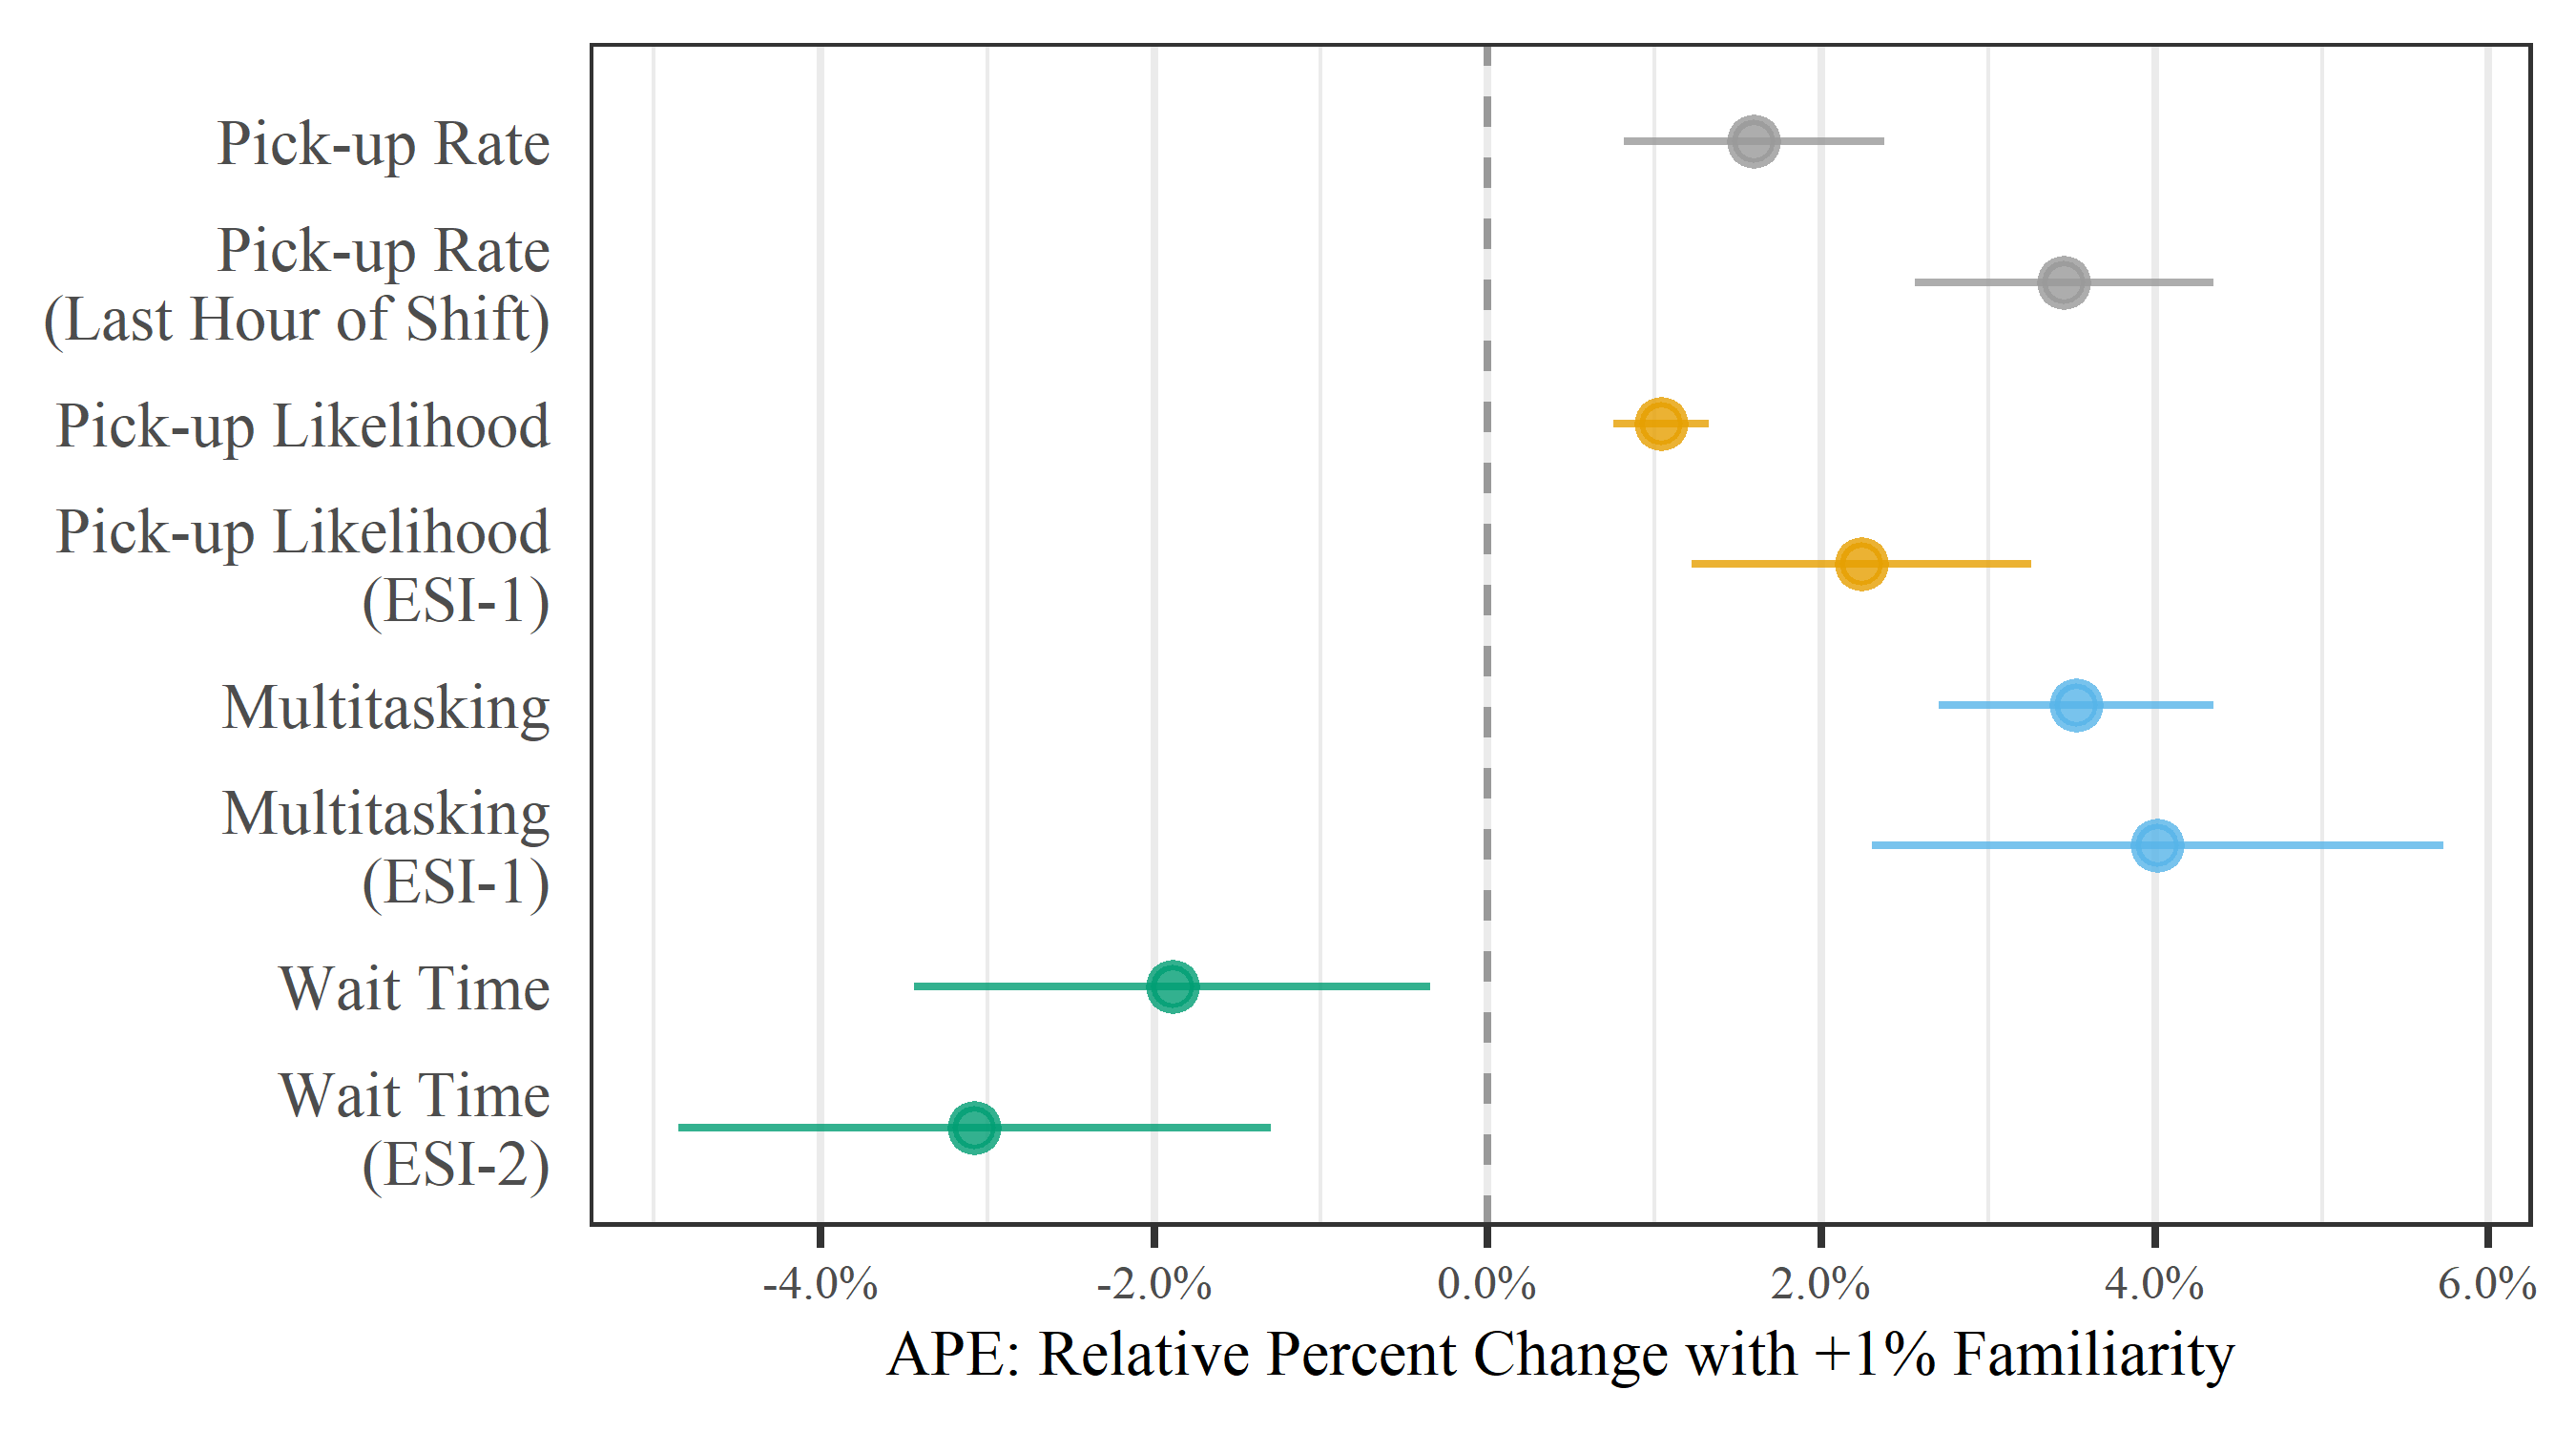
\includegraphics[scale=1]{Figures/PU/Post Hoc - Coef Plot.png}     
     \label{fig:pu_coef_plot}
     \floatfoot{\textit{Figure Note:} The figure illustrates how each measure would change (on average) with a 1\% increase in average familiarity. Percent changes for Pick-up Rate, Multitasking, and Wait Time are relative to median values in our dataset. For example, a 1\% increase in familiarity yields a 1.6\% increase in pick-up rate (relative to the median pick-up rate) on average, but the same increase in familiarity yields a 3.5\% increase in pick-up rate (relative to the median pick-up rate) during the last observed hour of the shift of a physician. Horizontal lines depict 95\% confidence intervals.}
 \end{figure} 
 
 We then asked: “If familiarity increases patient pick-up in the ED, what else changes with more familiarity?" When working among more familiar peers, we found physicians pick up patients at a faster rate and multitask more, and so one might expect patients also wait less. Encouragingly, we found patient wait time does decrease with familiarity. Similar to above, we find a stronger effect for ESI-2 patients (ESI-1 covers symptoms such as cardiac or respiratory arrest which must be treated immediately, regardless of familiarity). For such patients, a 1\% increase in familiarity yields a 1.57 minute decrease in patient waiting time ($p < 0.01$), or a 3.1\% decrease relative to the median waiting time of 51 minutes.
 
 Curiously, we found no effect of familiarity on patient processing time or length of stay. Even though patients experience shorter waits on average, the effect does not carry through to shorter visits overall. We do see one upside in such a result, however: Our findings might raise concerns if total patient length of stay increased even though wait time decreased. As \cite{KC2014} notes, the benefits of multitasking first diminish then reverse at higher levels of multitasking. KC notes the sweet-spot for multitasking seems to be around 4 to 5 patients -- exactly the range we observe in Figure \ref{fig:load_fam}. We find comfort in knowing the small, positive effect of familiarity does not seem to be accompanied by negative externalities.
 
 In all cases, within more familiar groups, physicians appear willing to exert more effort. Herein lies an important nuance: Physicians do not simply pick up more patients -- they pick up more severe patients, who are also likely to be more difficult cases. If physicians were only responding to social pressure to “work harder," then for the sake of appearance, they might pick up more easy patients. But picking up more difficult patients -- just to maintain an appearance -- seems unlikely. Furthermore, because the total effort spent treating patients in the ED is not fully observable, such prosocial behavior may go completely unrecognized, weakening such an extrinsic desire to conform. In all of our findings, patients in need of timely care stand to benefit the most as they wait less and are picked up more frequently. Our study explains how such benefits materialize and illustrates why researchers must consider server familiarity moving forward.

\section{Discussion \& Conclusion} \label{Conc_PU}
 As patient demand for emergency medicine grows, society will expect structural improvements and capacity investments to follow. But building new medical centers \citep{Woodworth2019,Li2021} or hiring more physicians represent time- and resource-intensive actions. We want to find alternatives which use resources managers already have, and simply deploy them better.
 
 In pursuit of such a goal, we consider a parallel server setting in the ED and explore how familiarity among physicians affects task selection and ultimately, multitasking. Familiarity is known to affect service rate \citep[e.g.,][]{Reagans2005}, and many jobs in service operations rely on some ability to multitask \citep[Section 5.1]{KC2020_productivity}. Building on such literature, we find familiarity affects multitasking, specifically through task selection which arises from individual discretion. Among ED physicians, greater average familiarity leads to (i) increased patient pick-up rate, (ii) observed multitasking, and (iii) shorter patient wait time -- all with (iv) no identifiable, negative impact to patient processing time or length of stay. Scheduling managers seeking to optimally redeploy resources should consider how staffing familiar servers together might alleviate capacity constraints with minimal additional cost.
 
 Our paper makes several \textbf{contributions} to the literature. First, by “bridging” the literature on queuing and the literature on familiarity, our study “prompts growth in all … contributing contexts” \citep[p. 732]{Reisman1995}. Traditionally the queuing literature ignores server familiarity and the familiarity literature ignores server discretion in task selection. We show familiarity affects task selection and the patient pick-up process, and modeling ED physicians in a vacuum omits the synergy of a physician cohort working together. Minimizing the effect of familiarity limits the literature's depth of insight because physicians have wide discretion to control how fast they work and how many patients they see. Our work addresses the limitation and shows the cumulative effect of such behavior on system-level outcomes.
 
 In monitoring physician behavior, we acknowledge our data does not reveal the full decision process of a physician. With patients waiting, an ED physician can choose to: (a) pick up a specific patient; (b) not pick up a patient, leaving him for another physician; or (c) see no more patients, ending her shift. We only observe scenarios (a) and (c) in our data. Future work should seek to better understand the full process where servers (physicians) may specifically overlook one task (patient) in favor of another. Additionally, although the ED provides a context to study familiarity among servers providing a vital service to society, our results only come from one setting. Therefore, future work should examine familiarity in other contexts to see if similar patterns hold.
 
 Second, our work is the first to explore familiarity impacting outcomes through task selection. Since (i) servers have discretion in task selection and (ii) we find familiarity affects task selection, then (iii) we expect familiarity impacts system-level outcomes through task selection. Indeed, we see discretion and task selection leads to shorter patient wait times. Our work shows familiarity shapes outcomes ignored by previous literature, and we demonstrate a channel through which it happens. We note one limitation of our research context here: In the ED, multitasking only changes with patient pick-up or discharge; in other contexts, multitasking might change through a variety of task selection decisions. But with our findings in hand, we encourage future research to build on the principle that familiarity affects such decisions.
 
 Third, in social exchange theory, we find a previously ignored behavioral driver for why familiarity affects task selection. Repeated exchanges in the ED build trust, cohesion, and an increased willingness to multitask. Unfortunately, our work cannot fully explain why familiarity affects our outcomes. Yes, physicians embrace multitasking, but perhaps they also accept longer shifts. We also do not observe the full degree of physician interaction in our data; we can count the number of patients picked up together, or the amount of time spent working together, but our measures only serve as a proxy for interactions. Future work should implement methods which more directly observe server collaboration, possibly with methodologies which isolate behavioral drivers better.
 
 Finally, we enhance our understanding of familiarity by identifying conditions where familiarity does, and does not, impact operational outcomes. For example, although familiarity leads to observed multitasking, we find no effect on patient processing time or length of stay. Such findings necessitate a holistic, systems-level approach: If we had simply measured multitasking at the physician-level, we would have missed broader implications for the system. In operations research, analytical models typify such an approach to operational outcomes. We see considerable value in empirical work continuing to leverage our insights to connect individual-level behaviors to the system-level outcomes, as urged by \cite{Allon2019}.
 
 Regrettably, despite our largely beneficial outcomes, we do not observe other patient health outcomes. We wonder: Can a busy physician overseeing several patients continue to provide the best level of care? Future work should incorporate more granular patient outcomes to generate more complete insights on the impact to patient health. 

 Our findings also generate several \textbf{managerial implications}. First, coworker familiarity may yield many benefits to a firm. To start, groups of familiar physicians multitask more with no detectable slowdowns elsewhere, thus reducing overcrowding. The increase in multitasking also leads to less patient wait time, where such time represents a strong determinant of patient experience \citep{Swallmeh2018}. Longer wait times also correspond to higher rates of patients leaving without being seen \citep{Shaikh2012} -– a subject of significant concern in both medicine and operations. Even further, familiarity significantly reduces the waiting time for the ED population with the greatest need (i.e., severe patients in urgent condition) -- a benefit for the firm and the patient. Picking up severe patients to maintain the appearance of “working hard” seems unlikely. Instead, we propose physicians lend familiar colleagues a hand by picking up patients most in need of care. Given budgetary constraints, a rising tide of patients, and a need to deliver a compelling patient experience, enabling familiarity offers a step in the right direction with minimal cost.

 Second, given the benefits, and since familiarity affects system-level outcomes, managers should seek to build familiarity through staffing decisions. For example, an optimal scheduling policy might consider staffing familiar servers together during the busiest hours to reduce wait time. Managers may even strategically staff unfamiliar workers together, paying the cost now to boost familiarity and foster resilience for the future. Nurturing familiarity takes time, but a system-level approach to staffing familiar workers together might yield substantial benefits. Future academic work should explore how to build and implement such staffing models.
 
 Finally, and perhaps most importantly, in situations where workers have discretion to choose what work they do, managers should think critically about task assignment. In our situation, firms benefit from increased multitasking, thanks to physician discretion. But discretion might also backfire \citep[e.g.,][]{Ibanez2017}, and familiarity \textit{variance} can undermine its own virtues \citep{Avgerinos2017}. Indeed, \cite{Ibanez2017} warn: “... discretion has costs that need to be balanced against its potential benefits" (p. 4404). Examples of critical questions include, “Do my employees have discretion in their choice of tasks? Will such discretion benefit or harm the system? Where beneficial, how can I encourage productive discretion? Where harmful, can I restrict discretion or -- at a minimum -- limit the negative consequences?" Our findings on familiarity and discretion have operational implications for all aspects of task design, including task training, sequencing, assignment, and especially server scheduling.
 
 In conclusion, we concur with \cite{KC2020_tcp}: “Our field studies many things, but work is central to what we do” (p. 4414). Operations research considers many facets of work: “\textit{What} work should we do? \textit{When} should we do it? And \textit{how} should we do it?” In our paper, we also ask, “\textit{Who} should be doing it?” The truth is who you work with matters, for both the individual and for the system. Our work provides some perspective on the role of familiarity among workers, and our insights empower future research to better identify the full spectrum of worker behavior in queues.